\documentclass[12pt]{article}

\usepackage[utf8]{inputenc}

\title{Rapid shortening at the eastern margin of the Tibetan plateau prior to the 2008 M_W=7.9 Wenchuan earthquake}
\author{T. Ben Thompson, Brendan J. Meade}
\date{September 2014}
\usepackage{graphicx}
\usepackage[margin=1.0in]{geometry}
\usepackage[nomarkers,figuresonly]{endfloat}
\usepackage{setspace}
\usepackage{natbib}
\doublespacing

\begin{document}

\maketitle

\section{Abstract}
The Longmen Shan is the steepest topographic front of the India-Asia collision and was the site of the $\textrm{M}_{\textrm{w}}$ 7.9  Wenchuan earthquake. Shortening estimates across the Longmen Shan provide strain accumulation rates and clarify the eastward extrusion of the Tibetan plateau. Here, to explain the interseismic GPS velocities across the greater Longmen Shan region, we develop a boundary element model including earthquake cycle effects, topography, the westward dipping Beichuan fault, and a $\sim 20$ km deep, shallowly dipping, detachment. The detachment is inferred from observations of slip during and after the Wenchuan earthquake and from structural considerations. Previous analyses which neglected the detachment and earthquake cycle effects have found shortening rates near zero. In contrast, we find that interseismic GPS data are consistent with a shortening rate of 5.7$\pm$1.5 mm/yr and maximum surface slip deficit rate of $NNN\pm NNN$ mm/yr. This model provides a unified interpretation of geodetic deformation throughout the earthquake cycle and is consistent and suggests that the Longmen Shan is an active fold-and-thrust belt with Wenchuan style earthquake recurrence intervals of $<$600 years.

\section{Introduction}
The Longmen Shan range is the steepest margin of the Tibetan Plateau rising 5 km over a distance of only 30 km at the western edge of the Sichuan Basin. In 2008 $\textrm{M}_{\textrm{w}}$ 7.9 Wenchuan earthquake ruptured the Beichan and Penguan rangefront thrust faults (over a distance $\sim 250$ km along strike) leading to approximately 70,000 earthquake related fatalities. GPS oberservations of co- and post-seismic deformation indicate slip not only on the steeply dipping Beichaun fault but also along a $\sim 20$ km deep sub-horizontal detachment surface extending an additional $\sim 100$ km west of the surface rupture. The inference of strain release associated with slip on an active detachment requires a complementary period of strain accumulation prior to the coseismic rupture. Interseismic GPS velocities measured prior to the occurence of the Wenchuan earthquake have been interpreted as indicating neglible \citep{king97, chen00, shen05, Meade07c, Loveless2011}. This apparent lack of present-day shortening across the steepest topography of the has been hypothesized to result from lower crustal inflation tectonic model for the eastern Tibetan Plateau (cite Clark and Royden papers)\citep{royden97, bird91, Burchfiel2008a}. However, these models do not provide a mechanism for accumulating the elastic strain released co- and post-seismically on the deep detachment to the west of the Beichuan fault \citep{Qi2011, Fielding2013b}.

Previous estimates of geodetically constrained shortening and slip deficit rates can be categorized into those that either: 1) do not explicitly treat earthquake cycle effects, \citep{chen00, shen05} (Thatcher too) or 2) those that use block models, with a first order approximation of earthquake cycle effects but coarse representations of fault system geometry \citep{Meade07c, Loveless2011, Burchfiel2008a}. Of these, the highest Longmen Shan rangefront slip deficit rates range up to 3.2 mm/yr \citep{Loveless2011}, as well as significant strain interior to the Longmen Shan block. Here, we present results from a two-dimensional boundary element models that includes earthquake cycle and topographic effects to explain the regional geodetic velocities that result from the combined effects of interseismic locking on both the range-front Beichuan fault and a 20 km deep detachment beneath the hinterland.  This fault system geometry is consistent with the inference of 2-6 m of slip of a 20 km deep detachment that extends 90 km northwest using InSAR measurements and post-Wenchuan GPS observations \citep{Qi2011, Fielding2013b} and interpretation of structural observations \citep{Hubbard2010, Li2010}. Integrating rangefront and detachment fault system geometry, we develop a model of interseismic strain accumulation that is consistent with both interseismic GPS velocities measured prior to the Wenchuan earthquake and previous observations of co- and post-seismic strain release at depth, and rapid slip deficit rates in the abscence of localized velocity gradients at the Longmen Shan rangefront.

\begin{figure}[h!]
    \centering
    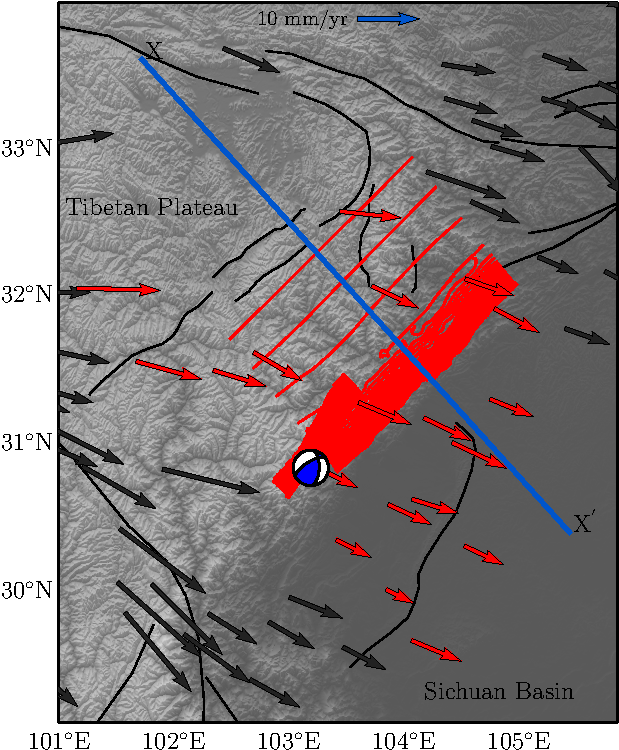
\includegraphics{figs/lms_map_all.pdf}
    \caption{Tectonic setting of the $\textrm{M}_{\textrm{w}}$ 7.9 Wenchuan earthquake and Longmen Shan rangefront. The focal mechanism is located at the epicenter of the Wenchuan earthquake and the thick red line shows the surface trace of rupture. The thin red lines show 1 km depth contours of the fault model. GPS velocity vectors (reference) are colored red if they are included in the two-dimensional models considered here. The blue line shows the two-dimensional cross-section we study. Thin black lines indicate other significant faults in the region \citep{Taylor09}.}
    \label{fig:regional_map}
\end{figure}

\section{Geodetic analysis of Longmen Shan shortening}
The geometry of the Beichaun fault and the detachment to the west have been inferred from 1) structural interpretations  \citet{Hubbard2010} (Plesch and Shaw, personal communication), 2) seismic relection observations (Ben, you found a paper for this where I misinterpreted the travel times as distances), and 3) geodetic modeling of co- and post-seismic deformation associated with the Wenchuan earthquake \citet{Qi2011, Fielding2013b}. The depth and dip of the detachment are similar to the best-fitting surface found by. The cross-section and geometry with depth contours are shown in Figure \ref{fig:regional_map}. The fault system geometry consists of two main segments. The range-front Beichuan fault dips steeply at $\sim 60^{\circ}$ at its surface trace shallowing to sub-horizontal near 20 km depth where it joins the detachment surface at depth. The detachment dips at $\sim 1.5^{\circ}$ from an initial depth of 20 km for 110 km to the northwest at its deepest point with a depth of 23 km. For the interseismic shortenging and slip deficit models considered here we consider an idealized two-dimensional representation of these fault surfaces (\ref{fig:regional_map}).

Because of the inference that the ~20 km deep detachment slipped, releasing elastic strain, either co- or post-seismically \citet{Qi2011} as distance >100 km to the west of the Beichaun fault, we include interseismic GPS velocities at similar distance into the interior of the Tibetan Plateau (Figure ref). We analyzed interseismic GPS velocities measured during the decade prior to the Wenchuan earthquake \citep{gan07}, in a nominally Eurasian reference frame \citet{apel06}. We exclude velocities that are near other major active structures including the Xianshuihe and Kunlun faults (Figure \ref{fig:regional_map}).

To model both the tectonic and earthquake cycle processes contributing to these interseismic GPS data, we use a quasistatic elastic boundary element software under active development. An important feature of our tool is the inclusion of accurate surface topography in steep mountainous regions or Earth curvature in large-scale problems. Previous boundary element methods in the earth sciences (cite thomas 93, maerten, etc) have been based on analytic integrations of rectangular or triangular slip surfaces (cite okada 92, meade 07). Developing these analytic formulae is time consuming. Analytic derivations normally assume an infinite half-space geometry and piecewise constant fault slip. To avoid these limitations, the basis for our boundary element formulation is numerical quadrature of the integrals in the elastic Somigliana identity (cite cruse 1969). The difficulty in this approach is that simple quadrature methods (for example, Gaussian quadrature) assume a smooth integrand. For observation points on or very close to a surface, including the free surface, the integrand is singular. We resolve this problem by evaluating singular integrals as the limit of a sequence of non-singular integrals. This approach is similar to analytical methods (Sutradhar et al. 2008) and the series-expansion quadrature by expansion (Klockner et al. 2013). Our tests of relative error show that this quadrature-based method can match, to arbitrary precision, analytically derived solutions and is free of the unpleasant singularities present in those solutions. This entirely numerical boundary element method allows for complete flexibility in surface geometry, including topography. In addition, we can accurately reproduce half-space solutions to very high precision (Quantify). The steep topography of the Longmen Shan range front is included via the SRTM30\_PLUS digital elevation dataset \citep{Becker2009}.

   Say what we actually solve for?  A single shortening rate which leads to the distribution of slip deficit rates.

To maintain kinematic consistency between the Sichuan Basin and Tibetan Plateau, we use a two-dimensional block formulation where the slip deficit rate on the fault, $s_\mathrm{sd}$, is related to the local fault dip, $\delta$, and total convergence rate, $v_0$, by $s_\mathrm{sd}=v_0 / cos\delta$ (Mccafrey 2002; Meade and Hager, 2005). The average interseismic slip deficit on the fault geometry is subtracted from block motion to calculate the interseismic velocity profile (Savage, 1983; Meade and Hager, 2005).

\begin{figure}[h!]
    \centering
    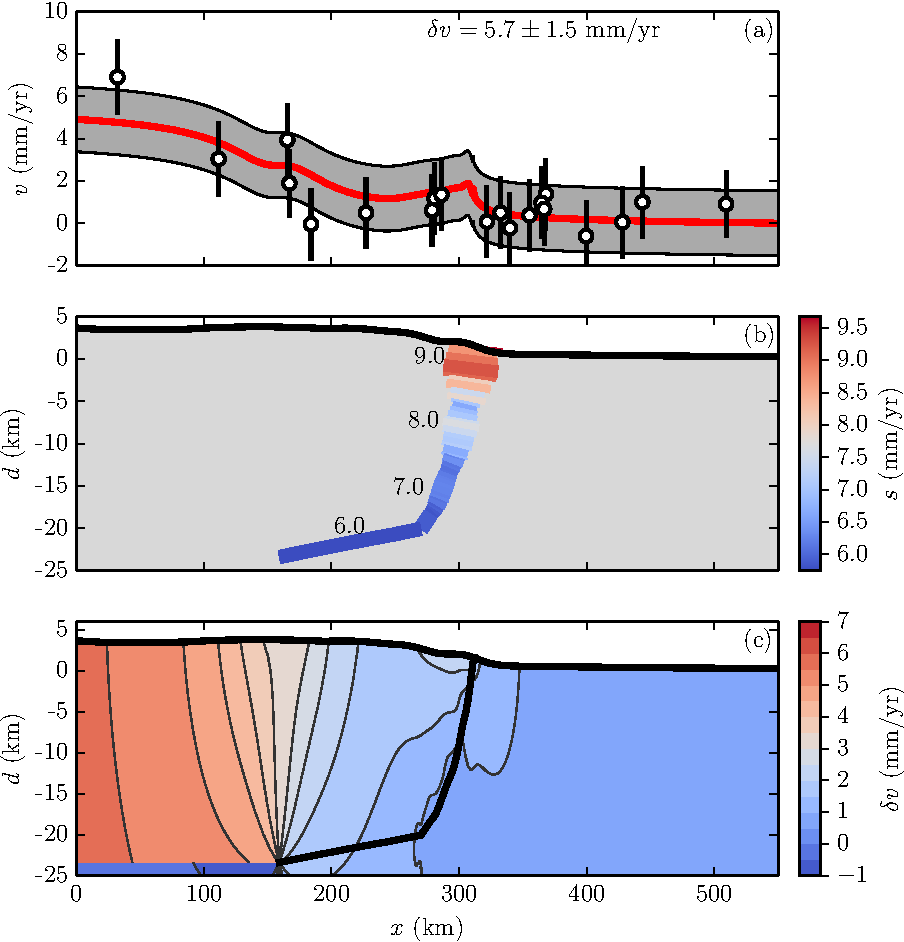
\includegraphics{figs/stack_figure_all_details.pdf}
    \caption{GPS velocities, model geometry, and inferend slip deficit rates. a) Observed profile-parallel horizontal observed velocities are shown in black with 68\% confidence errorbars. Model-predicted velocities are shown by the red line with the surrounding gray region showing a 68\% confidence interval. b) Model geometry with colors and width along the locked fault showing predicted slip-deficit rates. Because shortening is the horizontal component of slip-deficit, increasing dips near the surface lead to larger slip-deficits. c) Predicted horizontal velocity as a function of depth. Note the steep velocity gradient and corresponding strain accumulation above the end of the detachment surface. Vertical axes are exagerated in all panels.}
    \label{fig:big_stack}
\end{figure}

A Beichuan-only fault geometry (give approximate dip and locking depth) would predict <0.1 mm/yr of surface deformation at distances >100 km away from the fault trace \citep{savage83}. Both the observed and predicted profile-parallel velocities (Figure \ref{fig:big_stack}a) indicate that such an estimate would appear consistent with a near-zero slip deficit rate estimate and also fail to explain the co-/post-seismic slip on the detachment \citet{Qi2011, Fielding2013b}.

The inclusion of a locked detachment, however, shifts the predicted location of the steep interseismic velocity gradient far to the northwest (Figure \ref{fig:big_stack}a). When including a locked detachment, the least squares best-fit shortening rate for the Longmen Shan region is 5.7 $\pm$ 1.5 mm/yr. The spatial distribution of interseismic deformation is affected by the fault geometry and kinematic consistency constraints and represented in terms of the slip deficit rate which ranges shows the increase in slip-deficit from ~6.0 mm/yr on the deep detachment to 9.5 mm/yr at the surface trace of the Beichuan fault (Figure \ref{fig:big_stack}b). Figure \ref{fig:big_stack}c shows the horizontal velocities as a function of depth, demonstrating that the velocity gradients derive a locked to creeping transition at the detachment tip. The smoothing behavior of an elastic Earth prevents distinguishing between a sharp drop in slip-deficit or a gradual change over many kilometers. These results demonstrate a mechanism by which it is possible for interseismic strain accumulation to occur far from the range-front structures on which it is released.

The primary uncertainty in our shortening estimate is the lack of good constraints on the detachment geometry in the hinterland. However, assuming the geometry is correct, two further forms of error are evident. First, the uncertainty in true interseismic velocities is propagated through to the estimated shortening, resulting in the gray region of uncertainty in Figure \ref{fig:big_stack}a. Further, the sparsity of observations suggests that certain observations may have undue influence on the shortening estimate. Excluding the northwest-most observation decreases the best-fit shortening to 3.9 $\pm$ 1.9 mm/yr. (Add the range of slip deficit rates because the near surface Beichaun rate will still probably be close to 6 mm/yr).  The least squares uncertainty is increased (from 1.5 mm/yr to 1.9 mm/yr) because the northwestern portion of velocities are poorly constrained once the observation is excluded. This northwestern-most observation is adjacent to the Longriba fault, suggesting that it should not be included. However, the Longriba fault is primarily a dextral strike-slip fault \citep{Ren2013}, so it's influence should be predominantly orthogonal to the profile parallel velocities we examine here.

To quantify the sensitivity of slip deficit rate estimates to variability in data selection  we perform a complete case resampling bootstrap shortening and slip deficit rates are calculated for all possible subsets of the observed GPS velocities. There only $2^{20} = 1,048,576$ different possible subsets of the observations (Figure \ref{fig:distribution}). Subsequently, we sample jointly from this distribution and the distribution of surface-area weighted fault depths. This analysis demonstrates that the majority of the slip-deficit-depth probability landscape lies at slip-deficit rates between 4 and 6 mm/yr while certain parts of the geometry (the range-front) have much faster slip-deficit rates (give range of near surface rates). There is a non-negligible probability (give probability) assigned to slip-rates above 10 mm/yr in the steepest, near-surface portion of the fault system (Figure \ref{fig:distribution}). This is consistent with large near-surface coseismic slip (Quantify the max slip in any of the coseismic papers) during the Wenchuan earthquake \citep{Shen2009}. 

\begin{figure}[h!]
    \centering
    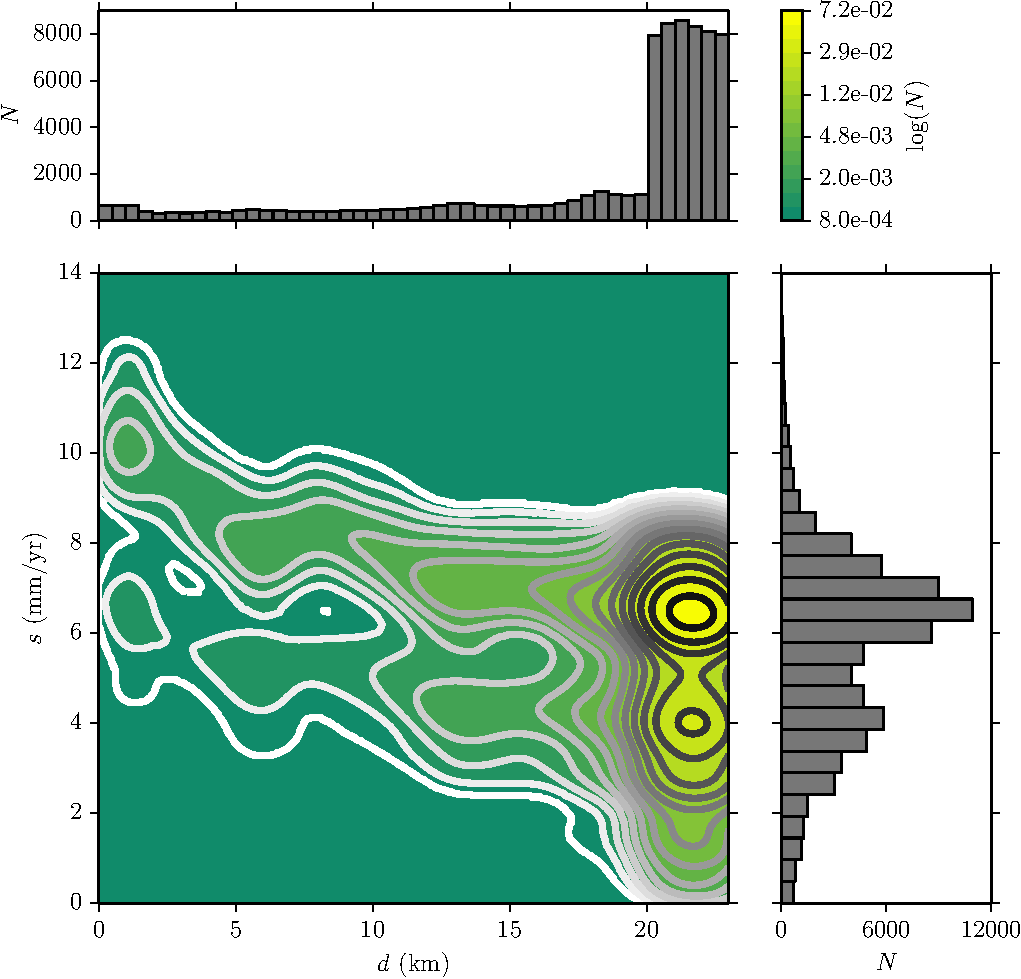
\includegraphics{figs/depth_slip_contour.pdf}
    \caption{The depth-slip-deficit probability landscape. The upper histogram is the projection of the contour plot onto a depth histogram, demonstrating that the majority of the fault surface area lies on the deep detachment. The right histogram is the projection of the contour plot onto a slip-rate histogram showing that the majority of fault surface area is slipping at rates near 6 mm/yr.}
    \label{fig:distribution}
\end{figure}

\section{Implications for the Longmen Shan earthquake cycle}
The fundamental effect of allowing a 20 km detachment to accumulated and release elastic strain through the earthquake cycle is the lack of a range-front geodetic signature despite the significant ($5-10$ mm/yr) slip deficit rate (\ref{fig:big_stack}a). Locking on the deep detachment obscures the signal of deformation on the range-front faults. The interseismic deformation is much more broadly distributed across more than 300 kilometers. According to this model, interseismically, the eastern Tibetan Plateau moves cohesively with the Sichuan Basin, whereas coseismic slip is concentrated at the boundary between these two blocks.

Prior analyses of interseismic deformation at the Longmen Shan including the effects of dipping fault system geometry and earthquake cycle effects have been limited (\citep{Loveless2011, Qi2011, Hao2014}). Of these only the three-dimensional block model of \citet{Loveless2011} is kinematically consistent (Jordan and Minster, McCaffrey, 2002; Meade and Hager, 2005). Compared to their estimated slip rate of 3.2 mm/yr, our estimate $2.5 \times$ as large.  Their calculations indicate a maximum 37\% likelihood of internal block strain west of the Longmen Shan region \citep{Loveless2011}. Attributing that block-internal strain to a deep detachment instead can explain the discrepancy between the two models. Our model of far-field deformation is also consistent with a similar detachment model of leveling and GPS-based uplift rates \citep{Hao2014}. The vertical velocities they measure increase from the Longmen Shan range front until peaking 50 km southeast of the Longriba fault zone at approximately 3.5 mm/yr of uplift. The Longriba fault zone has the wrong slip-sense (thrusting up to the south-east, \citep{Ren2013}) to accomodate such vertical deformation. No other identified structures are nearby. 

The velocity gradient which we link to the physics of the earthquake cycle and mapped fault system geometry has been alternatively asserted to represent distributed strain across the eastern Tibetan Plateau \citep{Royden2008}. Relatedly, \citet{kirby07} study an eastward decrease in interseismic velocities across the Kunlun fault. They conclude that the decline in slip-rate must be attributed to internal deformation. Further, fast erosion and inferred uplift rates have been used to support lower crustal inflation models in the absence of shortening \citep{Kirby2003}. All of these features can be explained with slip accomodated by a wide eastern Tibetan fold-and-thrust system, a suggestion supported by the continuation of shortening north from the Longmen Shan onto the Huya \citep{kirby00} and Min Jiang faults \citep{Chen1994}. In Figure \ref{fig:big_stack}c.

While we have explained the observed the broad GPS interseismic velocity gradient as a result of a locked detachment and the Beichaun fault we have not addressed when accumulated slip-deficit on the deep detachment is released. Geodetically constrained estimates of co- and post-seismic slip shows up to 5 m of slip on a deep detachment \citep{Qi2011}. Our data analysis depends on the detachment being locked during the period of data collection (when?). It is possible that in addition to coseismic and short-term postseismic activity on the detachment intermittent aseismic throughout the earthquake cycle could also be mode of strain release given that intersimsic GPS observations cover at best 6\% of a complete Longmen Shan earthquake cycle. Seismicity is approximately limited to the upper 20km of crust in the range-front \citep{Li2010}. Using steady-state critical taper wedge theory, we estimate a basal coefficient of friction between 0.02 and 0.30 (why does this vary so much?) for the detachment(cite Dahlen and give assumed pore fluid pressure and whether or not cohesion is assumed). The mean value of the coefficient of friction 0.05 is comparable to estimates of friction on the low-angle detachment system beneath the Longmen Shan foreland \citep{Hubbard2010}, indicating a very weak fault over long time-periods. On the other hand, the surface area and shortening rate of the detachment could sustain very large earthquakes if slip is released coseismically. Specifically, if 100km down-dip and 300km along-strike were to slip 4 meters, similar to average slip during the Wenchuan earthquake, a $M_{\textrm{w}}$ 8.4 rupture would be produced.

We also quantify the effect of explicitly treating surface topography by comparing models with and without surface topography, the local minimum in velocity (Figure \ref{fig:big_stack}a) northwest of the Beichuan is identified as the main topographically-influenced feature. The effects may be more pronounced with a shallower fault dip like in a subduction zones. Despite the mediocre effect (~15\%), geodetic analyses in steep regions should consider topographic effects to avoid systematic bias and these effects may be even more signficant for coseismic faulting cases where deformation is localized in regions of steep topography.

The 6-9 mm/yr slip deficit rates estimated here can be used to provide new constraints on earthquake recurrence intervals at the Longmen Shan (Figure \ref{fig:hazard}). Our shortening estimate suggests a recurrence interval for Wenchuan-like ruptures of approximately 600 years while recurrence intervals for smaller events would be more frequent. This contrasts with the average recurrence of ~2000 years inferred from paleoseismic field investigations for the Beichuan fault \citep{Ran2010}. The 6-9 mm/ry slip deficit rate estimated here would imply $M_{\textrm{w}} = $9.0 ruptures for that recurrence interval, which would seemingly require a along struke rupture equal to or greater than the $\sim 300$ km along strike length of the Longmen Shan, our slip deficit estimate could include the effects of other imbricated structures and thus serving as a system-wide estimate while paleoseismic estimates have been focused on the analysis of individual thrust faults. 

The earthquake recurrence intervals calculated above may be considered a lower bound for three reasons.  First, coseismic, interseismic, and long-term slip estimates include a significant component of strike-slip motion \citep{Shen2009, Qi2011, Densmore2007} (Meade2007, Loveless and Meade, 2011). while we consider an idealized case of fault normal motion only. Second, our two-dimensional model assumes plane strain conditions which will result in under-estimates of the shortening required to produce far-field velocities. This is because the assumption is equivalent to assuming the fault geometry extends infinitely far along strike. Third, the modeled thrust is the steeply dipping Beichuan fault. The foreland Range Front thrust or the shallow detachment beneath Chengdu dip more shallowly \citep{Hubbard2010}, producing a greater total moment deficit.  Finally, the slip deficit rate estimates may be low due to being estimated late in the earthquake cycle (i.e., in the decade prior to the Wenchuan earthquake) when viscoalstic relaxation effects may further contribute to a lowe near fault trace velocity gradient e.g., \citep{savage00}.

\begin{figure}[h!]
    \centering
    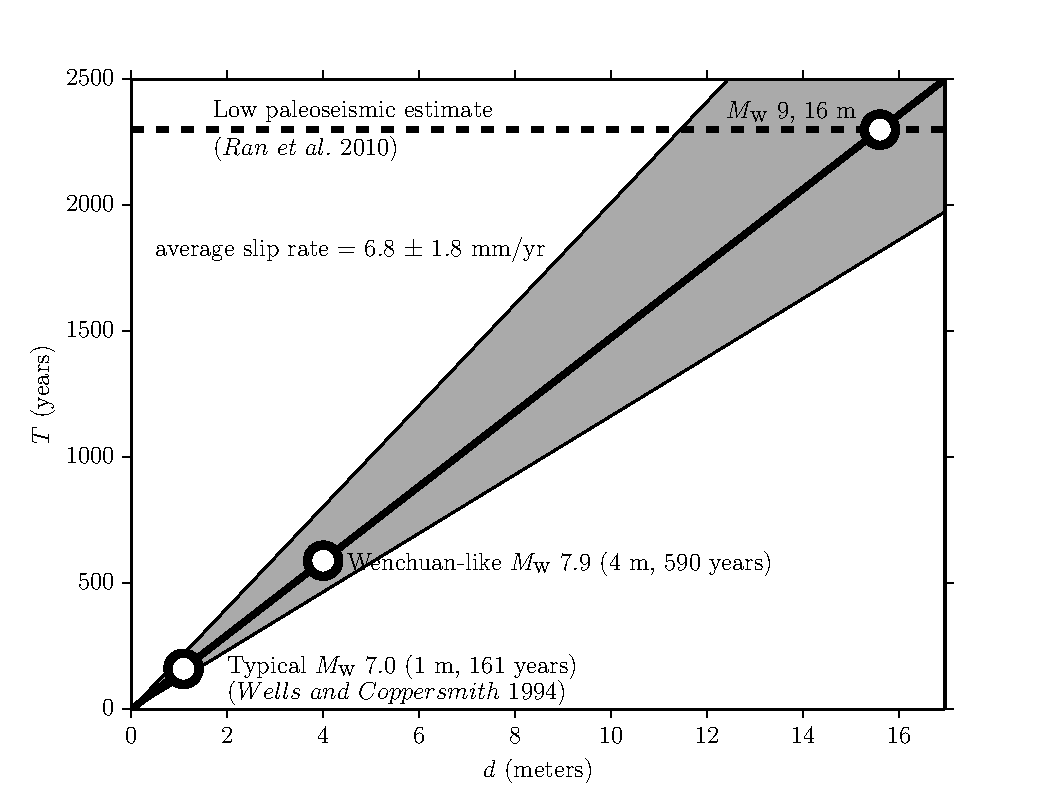
\includegraphics{figs/hazard_all_details.pdf}
    \caption{Earthquake recurrence intervals as a function of coseismic slip, assuming the best-fit slip rate for the Beichuan fault. The gray region indicates the uncertainty implied by the error in our shortening estimate. The discrepancy between the Wenchuan-like recurrence and the paleoseismic estimate may be due to the presence of multiple active faults in the range-front.}
    \label{fig:hazard}
\end{figure}

\section{Conclusion}
Previous inferences of near-zero interseismic shortening estimates at the Longmen Shan have been difficult to reconcile the Longmen Shan are at odds with the large-moment of the Wenchuan earthquake, very steep topography, structural interpretations indicate fold-and-thrust geometry, fast erosion rates. We offer a resolution to this conflict by including earthquake cycle effects associated with interseismic locking on the Beichuan fault and a 20 km deep detachment to the west. Our revised interseismic shortening rate is 5.7 $\pm$ 1.5 mm/yr with on fault slip-deficit rates up to 9.5 mm/yr near the surface, where the Beichuan fault is most steeply dipping. The model demonstrates that interseismic strain accumulation may be spatially disjoint from coseismic strain release, emphasizing that accurate fault system geometries are critical in the analysis of geodetic data. This boundary element model presented here unifies geodetic models of coseismic, postseismic and interseismic crustal deformation across the greater Longmen Shan region and suggests that, with current loading rates, Wenchuan-like earthquakes may recurrence as frequently as every 600 years.

\bibliographystyle{plainnat}
\bibliography{biblio,library}
\end{document}
